\documentclass[12pt, titlepage]{article}

\usepackage{graphicx}
\usepackage{booktabs}
\usepackage{amssymb}
\usepackage{xr}
\externaldocument[ext1-]{../../SRS/CA}
\externaldocument[ext2-]{../../Design/MG/MG}
\externaldocument[ext3-]{../../Design/MIS/MIS}
\externaldocument[ext4-]{../../VnVPlan/SystVnVPlan/SystVnVPlan}
\externaldocument[ext5-]{../../UserGuide/UserGuide}
\externaldocument[ext6-]{../../VnVPlan/UnitVnVPlan/UnitVnVPlan}
\usepackage{tabularx}
\usepackage{hyperref}
\hypersetup{
	colorlinks,
	citecolor=black,
	filecolor=black,
	linkcolor=red,
	urlcolor=blue
}
\usepackage[round]{natbib}
\newcommand{\myprogname}{Lattice Boltzmann Solver} 
%% Comments

\usepackage{color}

\newif\ifcomments\commentstrue

\ifcomments
\newcommand{\authornote}[3]{\textcolor{#1}{[#3 ---#2]}}
\newcommand{\todo}[1]{\textcolor{red}{[TODO: #1]}}
\else
\newcommand{\authornote}[3]{}
\newcommand{\todo}[1]{}
\fi

\newcommand{\wss}[1]{\authornote{blue}{SS}{#1}} 
\newcommand{\plt}[1]{\authornote{magenta}{TPLT}{#1}} %For explanation of the template
\newcommand{\an}[1]{\authornote{cyan}{Author}{#1}}


\begin{document}

\title{System Test Report: \myprogname} 
\author{Peter Michalski}
\date{\today}
	
\maketitle

\pagenumbering{roman}

\section{Revision History}

\begin{tabularx}{\textwidth}{p{3cm}p{2cm}X}
\toprule {\bf Date} & {\bf Version} & {\bf Notes}\\
\midrule
Dec. 16 & 1.0 & Initial Document\\
\bottomrule
\end{tabularx}

~\newpage

\section{Symbols, Abbreviations and Acronyms}

Please see Section \ref{ext1-CASYMBOLS} and Section \ref{ext1-CAABBACR} of the Commonality Analysis (\citet{LBM_CA_PM}).

\newpage

\tableofcontents

\listoftables %if appropriate

\listoffigures %if appropriate

\newpage

\pagenumbering{arabic}

This document reports the results of the tests found in the System VnV Plan (\citet{LBM_SVNV_PM}).

\section{Functional Requirements Evaluation}

Functional requirements are evaluated using system tests of id1A to id17 of the System VnV Plan (\citet{LBM_SVNV_PM}). Tests id11 to id17 are not covered in this report as they deal with a problem that is not implemented in the first stage of implementation of {\myprogname}. The results of tests id1A to id10 can be found in Section \ref{unittesting}. Traceability of the tests of this document to functional requirements is noted in Section \ref{traceabilitytoreq}. 

~\newpage

\section{Nonfunctional Requirements Evaluation}

\subsection{Maintainability}

This test will be conducted in January 2020.
		
\subsection{Performance}

System test id19 (performance-test-id19) found in Section \ref{ext4-secperf} of the System VnV Plan (\citet{LBM_SVNV_PM} compares the running time of each of the two problems, Von Karman Vortex Street and Poiseuille Flow, against the psuedo-oracle pyLBM using pyCharm IDE. The Poiseuille Flow problem will be tested in the second implementation of {\myprogname}. The test result for Von Karman Vortex Street is found below:


\begin{figure}[h!]
	\begin{center}
		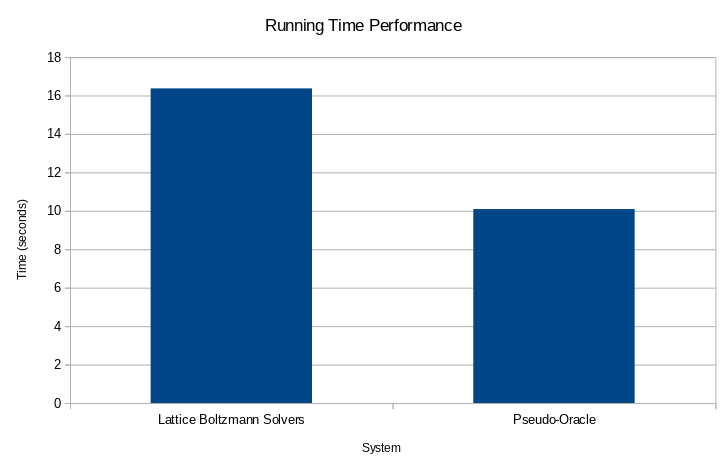
\includegraphics[width=1.0\textwidth]{runtimeperf}
		\caption{Running Time Performance of {\myprogname} vs Pseudo-Oracle}
		\label{Fig_RunningTimePerformance}
	\end{center}
\end{figure}

\noindent As we can see from Figure \ref{Fig_RunningTimePerformance}, the computational time of {\myprogname} is considerably longer (63\%) than that of the pseudo-oracle. This can be attributed to the increased overhead of {\myprogname}, which is designed for scalability with an increased number of libraries solving an increasing number of problems.

\subsection{Usability}

This test will be conducted in January 2020.
	
\section{Comparison to Existing Implementation}	
The first stage of implementation will not incorporate the Poiseuille Flow problem. Thus, Section \ref{ext4-frpf} of the System Vnv Plan (\citet{LBM_SVNV_PM}) is not reflected in this document.

\section{Unit Testing}
\label{unittesting}

\subsection{Input}
\subsubsection{input-reading-id1A}
\subsubsection{input-reading-id1B}
\subsubsection{input-bounds-id2A}
\subsubsection{input-bounds-id2B}

\subsection{Von Karman Vortex Street}
\subsubsection{tutorial-test-id3}
\subsubsection{Reynolds-rel-error-test-id4}
\subsubsection{laminar-test-id5}
\subsubsection{turbulent-test-id6}
\subsubsection{low-density-test-id7}
\subsubsection{high-density-test-id8}
\subsubsection{low-bulk-viscosity-test-id9}
\subsubsection{high-bulk-viscosity-test-id10}

\section{Changes Due to Testing}
No changes are necessary to the first stage of implementation due to these test results.

\section{Automated Testing}

The System VnV Plan (\citet{LBM_SVNV_PM}) specifies which unit tests were to be automated. Time constraints have resulted in manual testing of the tests reported in this document.
		
\section{Trace to Requirements}
\label{traceabilitytoreq}

A complete description of requirements is found in the CA (\citet{LBM_CA_PM}). A traceability of system tests to functional requirements can be found in Table \ref{ext4-Table:TRACFR} in Section \ref{ext4-tracereqs} of the System VnV Plan (\citet{LBM_SVNV_PM}). A traceability of system tests to NFRs can be found in Table \ref{ext4-Table:TRACNFR} of the same section.

\newpage

		
\section{Trace to Modules}	
\label{modulecoverage}

A complete description of modules is found in the MG (\citet{LBM_MG_PM}).

\begin{table}[!h]
	\begin{center}
		\begin{tabular}{| c | c | c | c | c | c | c | c | c | c | c | c | c | c |}
			\hline
			Cases / Modules & 1 & 2 & 3 & 4 & 5 & 6 & 7 & 8 & 9 & 10 & 11 & 12 & 13\\
			\hline
			id1A &\checkmark &\checkmark &\checkmark & & & & & & & & &\checkmark &\\
			\hline
			id1B &\checkmark &\checkmark & \checkmark& & & & & & & & & &\\
			\hline
			id2A &\checkmark & \checkmark&\checkmark & \checkmark& & & & & & & & \checkmark&\checkmark\\
			\hline
			id2B &\checkmark &\checkmark &\checkmark &\checkmark & & & & & & & &\checkmark &\checkmark\\
			\hline
			id3 &\checkmark &\checkmark &\checkmark & \checkmark & \checkmark& \checkmark&\checkmark & \checkmark& \checkmark&\checkmark & &\checkmark &\checkmark\\
			\hline
			id4 &\checkmark &\checkmark &\checkmark & \checkmark & \checkmark& \checkmark&\checkmark & \checkmark& \checkmark&\checkmark & &\checkmark &\checkmark\\
			\hline
			id5 &\checkmark &\checkmark &\checkmark & \checkmark & \checkmark& \checkmark&\checkmark & \checkmark& \checkmark&\checkmark & &\checkmark &\checkmark\\
			\hline
			id6 &\checkmark &\checkmark &\checkmark & \checkmark & \checkmark& \checkmark&\checkmark & \checkmark& \checkmark&\checkmark & &\checkmark &\checkmark\\
			\hline
			id7 &\checkmark &\checkmark &\checkmark & \checkmark & \checkmark& \checkmark&\checkmark & \checkmark& \checkmark&\checkmark & &\checkmark &\checkmark\\
			\hline
			id8 &\checkmark &\checkmark &\checkmark & \checkmark & \checkmark& \checkmark&\checkmark & \checkmark& \checkmark&\checkmark & &\checkmark &\checkmark\\
			\hline
			id9 &\checkmark &\checkmark &\checkmark & \checkmark & \checkmark& \checkmark&\checkmark & \checkmark& \checkmark&\checkmark & &\checkmark &\checkmark\\
			\hline
			id10 &\checkmark &\checkmark &\checkmark & \checkmark & \checkmark& \checkmark&\checkmark & \checkmark& \checkmark&\checkmark & &\checkmark &\checkmark\\
			\hline
			id11 &\checkmark &\checkmark &\checkmark & \checkmark & \checkmark& \checkmark&\checkmark & \checkmark& \checkmark&\checkmark & N/A &\checkmark &\checkmark\\
			\hline
			id12 &\checkmark &\checkmark &\checkmark & \checkmark & \checkmark& \checkmark&\checkmark & \checkmark& \checkmark&\checkmark & N/A &\checkmark &\checkmark\\
			\hline
			id13 &\checkmark &\checkmark &\checkmark & \checkmark & \checkmark& \checkmark&\checkmark & \checkmark& \checkmark&\checkmark & N/A &\checkmark &\checkmark\\
			\hline
			id14 &\checkmark &\checkmark &\checkmark & \checkmark & \checkmark& \checkmark&\checkmark & \checkmark& \checkmark&\checkmark & N/A &\checkmark &\checkmark\\
			\hline
			id15 &\checkmark &\checkmark &\checkmark & \checkmark & \checkmark& \checkmark&\checkmark & \checkmark& \checkmark&\checkmark & N/A &\checkmark &\checkmark\\
			\hline
			id16 &\checkmark &\checkmark &\checkmark & \checkmark & \checkmark& \checkmark&\checkmark & \checkmark& \checkmark&\checkmark & N/A &\checkmark &\checkmark\\
			\hline
			id17 &\checkmark &\checkmark &\checkmark & \checkmark & \checkmark& \checkmark&\checkmark & \checkmark& \checkmark&\checkmark & N/A &\checkmark &\checkmark\\
			\hline
			id18 &\checkmark &\checkmark &\checkmark & \checkmark & \checkmark& \checkmark&\checkmark & \checkmark& \checkmark&\checkmark & \checkmark &\checkmark &\checkmark\\
			\hline
			id19 &\checkmark &\checkmark &\checkmark & \checkmark & \checkmark& \checkmark&\checkmark & \checkmark& \checkmark&\checkmark & \checkmark &\checkmark &\checkmark\\
			\hline
			id20 &\checkmark &\checkmark &\checkmark & \checkmark & \checkmark& \checkmark&\checkmark & \checkmark& \checkmark&\checkmark & \checkmark &\checkmark &\checkmark\\
			\hline
		\end{tabular}
		\caption{Traceability Matrix Showing the Connections Between Test Cases and Modules}
		\label{Table:MODCOV}
	\end{center}
\end{table}  	

~\newpage

\section{Code Coverage Metrics}

Module coverage is guaranteed for those modules that are implemented and not outsourced to external libraries. Module coverage is outline in Table \ref{Table:MODCOV} of Section \ref{modulecoverage}.

~\newpage

\bibliographystyle {plainnat}
\bibliography {../../../refs/References}

\end{document}